% Taller 4 -- Lógica difusa (robot). Compilar:
% tectonic -Z search-path=$HOME/repos/ud/maestria/mcic/.UniversidadDistrital-manual-marca/plantillas-latex informe_taller4.tex
% Las cifras salen de taller4_robot_difuso.ipynb ejecutado.
\documentclass[11pt,letterpaper]{article}
\usepackage{ud-informe}
\usepackage{amsmath}
\usepackage{qrcode}
\colorlet{udrojo}{udazul}
\definecolor{udrojoosc}{HTML}{0C6F96}

\renewcommand{\UDtitulo}{Clasificador difuso para la navegación de un robot}
\renewcommand{\UDsubtitulo}{Modelos de 2 y 4 sensores con funciones de pertenencia leídas del análisis de datos}
\renewcommand{\UDtipo}{Taller 4 -- Informe}
\renewcommand{\UDasignatura}{Inteligencia Computacional Aplicada}
\renewcommand{\UDdocente}{Cesar Andrey Perdomo Charry}
\renewcommand{\UDestudiantes}{Juan Felipe Rodríguez Galindo -- 20261595004}
\renewcommand{\UDencabezado}{Taller 4 -- Lógica difusa (robot)}

% Enlace del video de la grabación
\newcommand{\VIDEO}{https://youtu.be/VNrNky4D76U}

\begin{document}
\UDportada

\section{Introducción}

A partir del análisis empírico de los movimientos de un robot móvil, en este taller construí dos modelos de lógica difusa para clasificar su maniobra de navegación: uno basado en 2 sensores frontolaterales y otro extendido a 4, deduciendo las funciones de pertenencia desde los histogramas globales, la distribución condicionada por clase y la dispersión en nube de puntos, respetando el límite máximo de 100 reglas.

El conjunto de datos registra lecturas continuas de ultrasonido provenientes de un robot seguidor de pared (\texttt{sensor\_readings\_2.csv} y \texttt{sensor\_readings\_4.csv}, sin cabeceras), midiendo distancias en metros hacia la pared por el frente, la izquierda, la derecha y la parte posterior junto a una de cuatro acciones posibles: avanzar (\textit{Move-Forward}), giro fuerte a la derecha (\textit{Sharp-Right-Turn}), giro leve a la izquierda (\textit{Slight-Left-Turn}) y giro leve a la derecha (\textit{Slight-Right-Turn}).

Entregables: el cuaderno \texttt{taller4\_robot\_difuso.ipynb} ejecutado, los dos CSV, \texttt{requirements.txt} y este informe; antes de programar formulé el plan y mis hipótesis, quedando todo el desarrollo grabado en video (sección~\ref{sec:ia}).

\section{Marco teórico}

\textbf{Funciones de pertenencia trapezoidales.} Un conjunto difuso mapea cada valor continuo a un grado de pertenencia en $[0,1]$, donde la función trapezoidal $\mathrm{trapmf}(x;a,b,c,d)$ asciende linealmente de 0 en $a$ a 1 en $b$, permanece en meseta unitaria entre $b$ y $c$, y desciende a 0 en $d$:
\begin{equation*}
\mathrm{trapmf}(x;a,b,c,d)=\max\!\left(0,\ \min\!\left(\frac{x-a}{b-a},\ 1,\ \frac{d-x}{d-c}\right)\right).
\end{equation*}
Fijando $a=b$ o $c=d$ la curva queda abierta hacia el extremo respectivo, permitiendo modelar adecuadamente etiquetas semánticas extremas como ``cerca'' (iniciando en 0) o ``lejos'' (alcanzando los 5\,m de cota física del sensor).

\textbf{Reglas y t-norma producto.} Cada regla difusa sigue la estructura condicional ``SI frontal es $A_1$ Y izquierda es $A_2$ \dots{} ENTONCES clase $=k$'', calculándose la activación de la regla mediante el producto algebraico de sus antecedentes, $\prod_j \mu_{A_j}(x_j)$; cada observación se clasifica asignándola a la regla que ostente el mayor grado de disparo.

\textbf{Número de reglas.} Al disponer de $m$ conjuntos difusos por cada una de las $n$ variables de entrada se generan teóricamente $m^n$ combinaciones; así, con 3 particiones semánticas surgen $3^2=9$ reglas para el esquema de 2 sensores y $3^4=81$ para el de 4 entradas, manteniéndose ambos por debajo de la restricción de 100 reglas.

\section{Metodología}

\textbf{Entorno.} El pipeline se implementó en Python 3.12 gestionado con \texttt{uv}, empleando numpy, pandas, matplotlib y scikit-learn (exclusivamente para la partición y cálculo de matrices de confusión); el motor de inferencia y la evaluación matemática de pertenencia se programaron directamente en el cuaderno. Los parámetros globales como la semilla aleatoria (\texttt{SEMILLA = 42}), el porcentaje de prueba (\texttt{PRUEBA = 0.3}) y las rutas de lectura se parametrizaron en la cabecera.

\textbf{Datos.} Ambos ficheros contienen 5456 observaciones; tras verificar que los campos de frontal, izquierda y etiqueta en \texttt{sensor\_readings\_4.csv} replican con exactitud los de \texttt{sensor\_readings\_2.csv}, se aplicó una partición estratificada 70-30 común: 3819 instancias para entrenamiento y 1637 para prueba. El conjunto refleja un marcado desbalance de clases (2205 muestras de avance, 2097 de giro fuerte a derecha, 826 de giro leve a derecha y 328 de giro leve a izquierda), por lo que la partición es estratificada; además, todo el análisis exploratorio y ajuste de trapecios se restringió estrictamente al subconjunto de entrenamiento para no filtrar información de la prueba.

\textbf{Funciones de pertenencia.} Se fijaron tres particiones por sensor (cerca, media, lejos) con zonas de solapamiento gradual de 10 a 20\,cm alrededor de los umbrales identificados (tabla~\ref{tab:mf}); en frontal e izquierda los puntos de corte provienen directamente de los histogramas por clase, mientras que en derecha y atrás, al presentarse una dispersión indiferenciada, los cortes se derivaron de los terciles del entrenamiento.

\textbf{Reglas.} En lugar de definir las reglas a priori, el sistema sintetiza las combinaciones posibles y asocia a cada antecedente la clase mayoritaria que maximiza el soporte en entrenamiento mediante $\sum_{i:\,y_i=k} \prod_j \mu_{A_j}(x_{ij})$; dicha métrica cuantifica el respaldo empírico de cada regla y hace explícita su consistencia con los datos observados.

\section{Análisis de datos}

La figura~\ref{fig:hist} ilustra la distribución de distancias registradas por cada sensor, evidenciando en los cuatro casos colas prolongadas hacia los 5\,m (límite operativo del sensor) con la gran mayoría de mediciones concentradas bajo los 3\,m.

\begin{figure}[H]
\centering
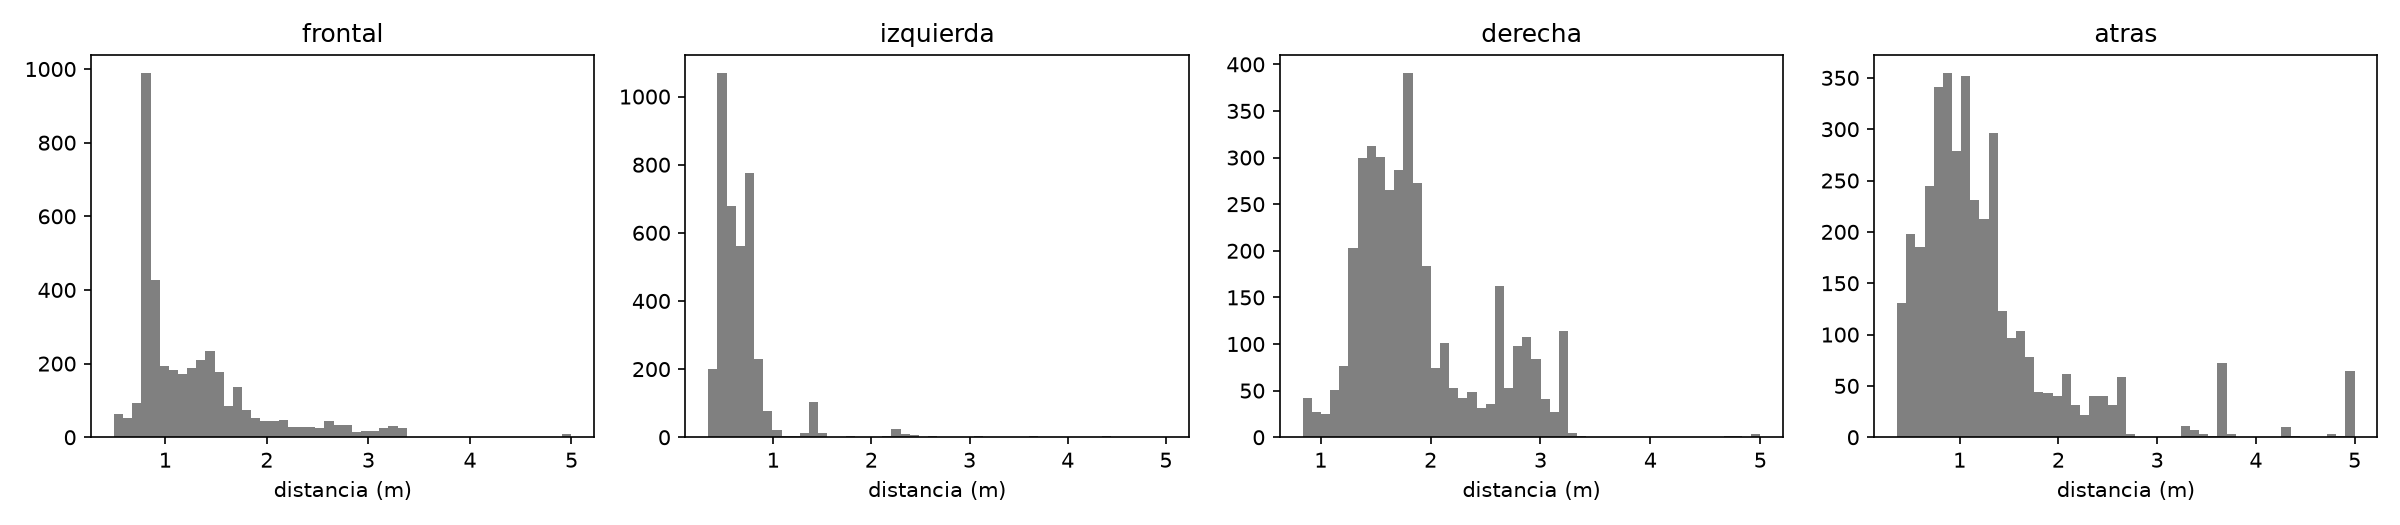
\includegraphics[width=\linewidth]{../figuras/histogramas.png}
\caption{Histogramas de los cuatro sensores (entrenamiento).}\label{fig:hist}
\end{figure}

El comportamiento condicionado por maniobra (figura~\ref{fig:histclase}) constituye el núcleo del diagnóstico:
\begin{itemize}
\item \textbf{Frontal:} la totalidad de los giros fuertes a la derecha se restringe a valores inferiores a 0,9\,m sin que ninguna otra acción descienda de dicha cota; ante cualquier obstáculo frontal próximo el robot ejecuta indefectiblemente un viraje cerrado.
\item \textbf{Izquierda:} el giro leve a derecha se confina por debajo de 0,5\,m al encontrarse la unidad excesivamente arrimada al muro, mientras el giro leve a izquierda se activa por encima de 0,9\,m al distanciarse de este; la maniobra de avance ocupa justamente la franja intermedia entre 0,5 y 0,9\,m.
\item \textbf{Derecha y atrás:} las distribuciones de las cuatro acciones se solapan prácticamente en su totalidad, observándose únicamente en el sensor trasero una leve inclinación del giro leve izquierdo hacia lecturas elevadas.
\end{itemize}

\begin{figure}[H]
\centering
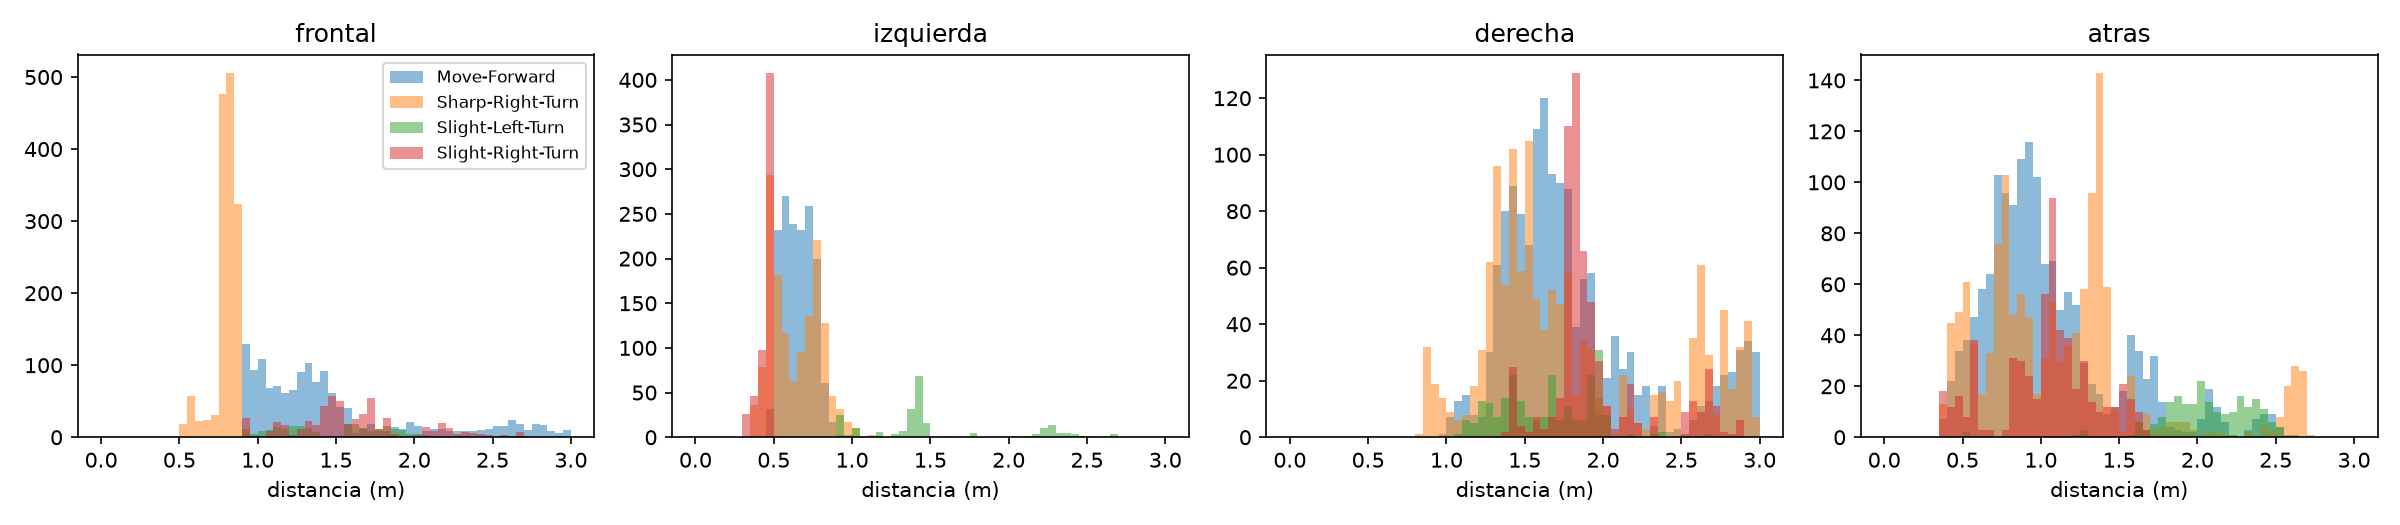
\includegraphics[width=\linewidth]{../figuras/histogramas_clase.png}
\caption{Histogramas por clase de los cuatro sensores (entrenamiento, 0 a 3\,m).}\label{fig:histclase}
\end{figure}

La proyección bidimensional (figura~\ref{fig:nube}) ratifica este patrón: sobre el plano frontal--izquierda las clases demarcan regiones bien delimitadas, casi rectangulares, mientras en el espacio derecha--atrás lucen completamente entremezcladas; consecuentemente, para estas dos variables se tomaron los terciles del entrenamiento como umbrales (1,57 y 1,92\,m en derecha; 0,87 y 1,30\,m en atrás).

\begin{figure}[H]
\centering
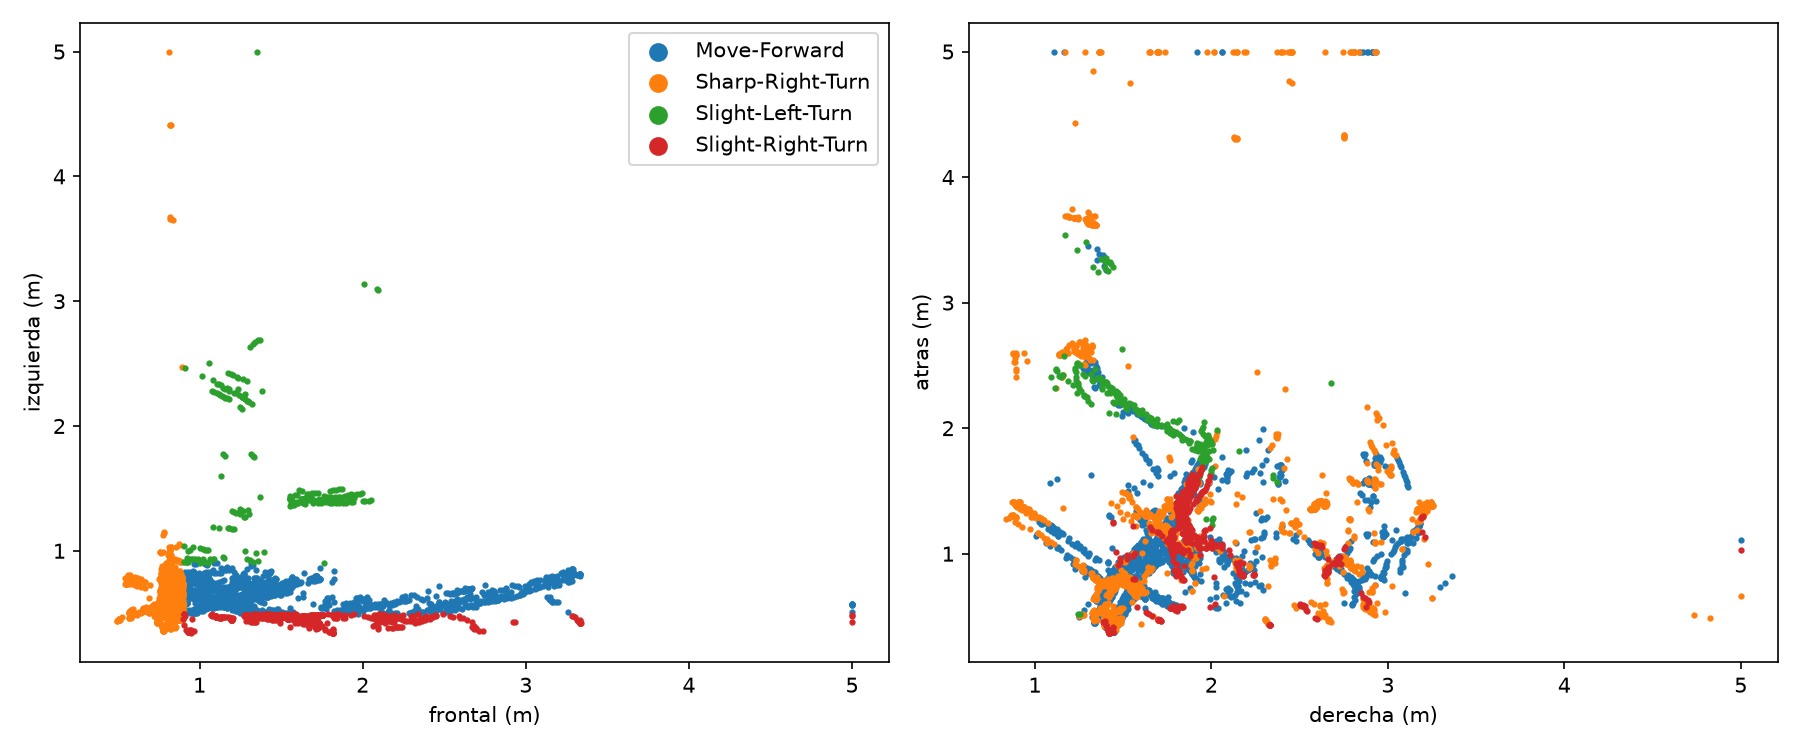
\includegraphics[width=\linewidth]{../figuras/nube_puntos.png}
\caption{Nube de puntos del entrenamiento: frontal contra izquierda y derecha contra atrás.}\label{fig:nube}
\end{figure}

\begin{table}[H]
\centering
\caption{Funciones de pertenencia trapezoidales $(a,b,c,d)$ en metros.}\label{tab:mf}
\begin{tabular}{lccc}
\toprule
Sensor & Cerca & Media & Lejos \\
\midrule
Frontal & $(0,\ 0,\ 0{,}85,\ 0{,}95)$ & $(0{,}85,\ 0{,}95,\ 1{,}6,\ 2{,}0)$ & $(1{,}6,\ 2{,}0,\ 5,\ 5)$ \\
Izquierda & $(0,\ 0,\ 0{,}48,\ 0{,}52)$ & $(0{,}48,\ 0{,}52,\ 0{,}85,\ 0{,}95)$ & $(0{,}85,\ 0{,}95,\ 5,\ 5)$ \\
Derecha & $(0,\ 0,\ 1{,}47,\ 1{,}67)$ & $(1{,}47,\ 1{,}67,\ 1{,}82,\ 2{,}02)$ & $(1{,}82,\ 2{,}02,\ 5,\ 5)$ \\
Atrás & $(0,\ 0,\ 0{,}77,\ 0{,}97)$ & $(0{,}77,\ 0{,}97,\ 1{,}2,\ 1{,}4)$ & $(1{,}2,\ 1{,}4,\ 5,\ 5)$ \\
\bottomrule
\end{tabular}
\end{table}

\begin{figure}[H]
\centering
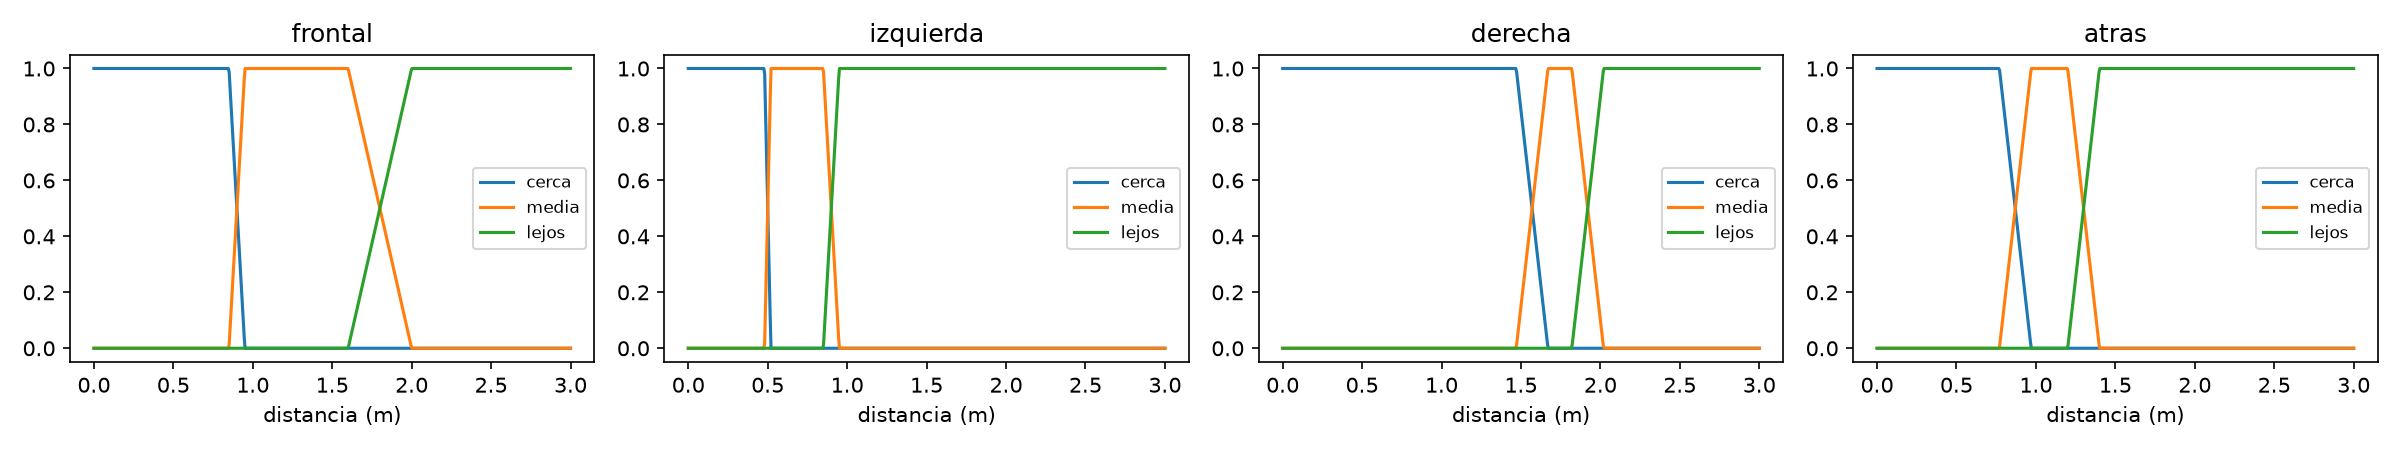
\includegraphics[width=\linewidth]{../figuras/funciones_pertenencia.png}
\caption{Funciones de pertenencia de cada sensor (mostradas de 0 a 3\,m).}\label{fig:mf}
\end{figure}

\section{Resultados}

\subsection{Modelo de 2 sensores}

Las 9 reglas generadas cuentan con soporte directo en entrenamiento (tabla~\ref{tab:reglas2}), logrando una exactitud del 98,96\,\% sobre el conjunto de prueba al clasificar 1620 de las 1637 lecturas evaluadas.

\begin{table}[H]
\centering
\caption{Las 9 reglas del modelo de 2 sensores con su soporte en el entrenamiento.}\label{tab:reglas2}
\begin{tabular}{llll}
\toprule
Frontal & Izquierda & Acción & Soporte \\
\midrule
cerca & cerca & Sharp-Right-Turn & 380 \\
cerca & media & Sharp-Right-Turn & 975 \\
cerca & lejos & Sharp-Right-Turn & 77 \\
media & cerca & Slight-Right-Turn & 441 \\
media & media & Move-Forward & 1155 \\
media & lejos & Slight-Left-Turn & 180 \\
lejos & cerca & Slight-Right-Turn & 179 \\
lejos & media & Move-Forward & 384 \\
lejos & lejos & Slight-Left-Turn & 48 \\
\bottomrule
\end{tabular}
\end{table}

\subsection{Modelo de 4 sensores}

De las 81 reglas posibles, 73 hallan respaldo muestral en entrenamiento (18 para avanzar, 30 para giro fuerte a la derecha, 12 para giro leve a la izquierda y 13 para giro leve a la derecha), correspondiendo las 8 restantes a combinaciones no observadas en la trayectoria; este modelo alcanza un 98,90\,\% de acierto en prueba (1619 de 1637 lecturas).

\subsection{Comparación}

La tabla~\ref{tab:comp} resume los dos modelos y la tabla~\ref{tab:conf} muestra sus matrices de confusión.

\begin{table}[H]
\centering
\caption{Comparación de los dos modelos en las 1637 lecturas de prueba.}\label{tab:comp}
\begin{tabular}{cccc}
\toprule
Sensores & Reglas & Exactitud & Errores \\
\midrule
2 & 9 & 98,96\,\% & 17 \\
4 & 81 (73 con soporte) & 98,90\,\% & 18 \\
\bottomrule
\end{tabular}
\end{table}

\begin{table}[H]
\centering
\caption{Matrices de confusión en prueba (filas: clase real; columnas: predicha; MF = Move-Forward, SR = Sharp-Right-Turn, LL = Slight-Left-Turn, LR = Slight-Right-Turn).}\label{tab:conf}
\begin{tabular}{l|cccc|c}
\multicolumn{6}{c}{\textbf{2 sensores}} \\
\toprule
 & MF & SR & LL & LR & Sensibilidad \\
\midrule
MF & 648 & 0 & 0 & 14 & 97,9\,\% \\
SR & 2 & 626 & 0 & 1 & 99,5\,\% \\
LL & 0 & 0 & 98 & 0 & 100\,\% \\
LR & 0 & 0 & 0 & 248 & 100\,\% \\
\bottomrule
\end{tabular}
\qquad
\begin{tabular}{l|cccc|c}
\multicolumn{6}{c}{\textbf{4 sensores}} \\
\toprule
 & MF & SR & LL & LR & Sensibilidad \\
\midrule
MF & 648 & 0 & 0 & 14 & 97,9\,\% \\
SR & 2 & 626 & 0 & 1 & 99,5\,\% \\
LL & 0 & 0 & 98 & 0 & 100\,\% \\
LR & 0 & 1 & 0 & 247 & 99,6\,\% \\
\bottomrule
\end{tabular}
\end{table}

Ambas arquitecturas coinciden en su veredicto en 1636 de las 1637 lecturas de prueba; la única discrepancia concierne a un giro leve a la derecha que la versión de 4 sensores reclasifica erróneamente como giro fuerte.

\section{Análisis}

\textbf{Frontal e izquierda deciden.} Los histogramas y la nube de dispersión anticipaban que las lecturas de derecha y atrás carecen de poder discriminante, corroborándose plenamente en los resultados: incorporar ambos sensores multiplica la base de reglas por un factor de 9 (escalando de 9 a 81) sin aportar beneficio en exactitud. Al agrupar las 73 reglas activas del modelo cuádruple según su par frontal--izquierda, 7 de las 9 combinaciones replican idéntica acción a la del modelo de 2 sensores; de hecho, los dos sensores adicionales solo alteran la decisión en dos combinaciones (frontal media con izquierda próxima o distante), donde en lugar de subsanar fallos terminan introduciendo una clasificación errónea.

\textbf{Los errores residen en los bordes.} Las 17 discrepancias del modelo de 2 sensores se localizan sobre las fronteras de corte; en particular, 15 lecturas sitúan la izquierda entre 0,491 y 0,500\,m donde ``cerca'' y ``media'' compiten en pertenencia cuasi-idéntica (14 avances confundidos como giros leves a la derecha y 1 giro fuerte), mientras las 2 restantes corresponden a giros fuertes con frontal en 0,90\,m rotulados como avance. Al ser los cortes en los datos extremadamente abruptos, el rango de transición difuso reparte el grado entre conjuntos contiguos y la regla equivocada prevalece por un margen mínimo.

\textbf{Avanzar es la maniobra más comprometida.} Su menor sensibilidad (97,9\,\%) obedece a que ocupa el corredor central del sensor izquierdo compartiendo ambos flancos con los giros correctivos; en contraposición, las maniobras de giro leve, pese a su baja frecuencia muestral, se aíslan sin dificultad al asentarse sobre los extremos exteriores de la distribución.

\textbf{Sentido físico de las reglas.} La base de 9 reglas reproduce la lógica natural de un seguimiento de pared lateral izquierda: ante una obstrucción frontal inminente el robot vira fuertemente a la derecha; cuando el flanco izquierdo se arrima en exceso ejecuta una corrección suave a la derecha; si se aparta demasiado gira levemente hacia la izquierda para retomar referencia; y con el frente despejado y la pared a distancia prudente, sostiene el avance.

\textbf{Hipótesis contra resultados.} En la planificación previa planteé cuatro interrogantes:
\begin{enumerate}
\item \textit{¿Qué sensores separan mejor las clases?} Anticipé ``4 sensores'', pero no se cumplió: frontal e izquierda concentran la discriminación y los demás se superponen.
\item \textit{¿El modelo de 4 sensores será mejor que el de 2?} Supuse afirmativamente, pero no se verificó: con 9 reglas el modelo base rindió 98,96\,\%, mientras 81 reglas apenas dieron 98,90\,\%.
\item \textit{¿Qué clase será la más difícil de clasificar?} Indiqué ``CD CI CF CA'' de forma genérica; el experimento demostró que avanzar fue la más exigente, concentrando 14 de los fallos de prueba.
\item \textit{¿Las reglas aprendidas tendrán sentido físico para el robot?} Contesté ``Sí'' y se confirmó cabalmente al describir un comportamiento coherente de navegación por pared izquierda.
\end{enumerate}

\section{Conclusiones}

\begin{enumerate}
\item La exploración estadística reveló fronteras operativas nítidas en entrenamiento: frontal en 0,9\,m para el viraje fuerte, e izquierda en 0,5 y 0,9\,m para las correcciones leves, demostrando que derecha y atrás no aportan información clasificatoria útil.
\item Ajustando trapecios en torno a estos umbrales, el modelo de 2 sensores precisa únicamente 9 reglas para alcanzar un 98,96\,\% de exactitud sobre el conjunto de prueba.
\item La arquitectura de 4 sensores expande la complejidad a 81 reglas para obtener un 98,90\,\%; incorporar más entradas no aportó mejoras al carecer de poder discriminante.
\item Los fallos se concentran sobre los límites de transición semántica, predominantemente en lecturas izquierdas próximas a 0,5\,m, siendo avanzar la acción más sensible al solapamiento.
\item La base de reglas sintetizada preserva plena interpretabilidad y se traduce directamente en comandos ejecutables de seguimiento de pared por el flanco izquierdo.
\end{enumerate}

\section{Declaración de uso de IA}\label{sec:ia}

Usé Claude (Anthropic) para revisar y corregir errores y para redactar este informe a partir de los resultados del cuaderno. Todo el desarrollo quedó grabado:

\begin{center}
\qrcode[height=3.2cm,nolink]{https://youtu.be/VNrNky4D76U}\\[0.6em]
\url{https://youtu.be/VNrNky4D76U}
\end{center}

\end{document}
